%%%%%%%% Capitolo3 %%%%%%%%
\chapter{Caratterizzazione dei materiali}
\label{chap:risultati}

\section[Quantum Dots]{\emph{Quantum Dots}}
 Qui di seguito sono riportati i risultati delle caratterizzazioni FT-IR, UV-vis, fotoluminescenza, DLS (\emph{Dynamic Light Scattering}), 
 $^{31}$P-NMR e TEM eseguite sulle nanoparticelle di CdSe passivate con leganti TOPO (tri-ottilfosfina ossido) e TDPA (acido 1-tetradecilfosfonico).

{
Confrontando gli spettri FT-IR in~\ref{fig:CdSe-TOPO_TDPA-IR-TOPO_TDPA} possiamo osservare che il debole picco dello \emph{stretching} P=O a 1125~cm$^{-1}$ si sposta a 1101~cm$^{-1}$ in presenza delle nanoparticelle, questo può essere attribuito alla coordinazione del gruppo fosfonico al CdSe tramite l'ossigeno P=O  \cite{lig-CdSe-caratt}}. 

\begin{figure}
\centering{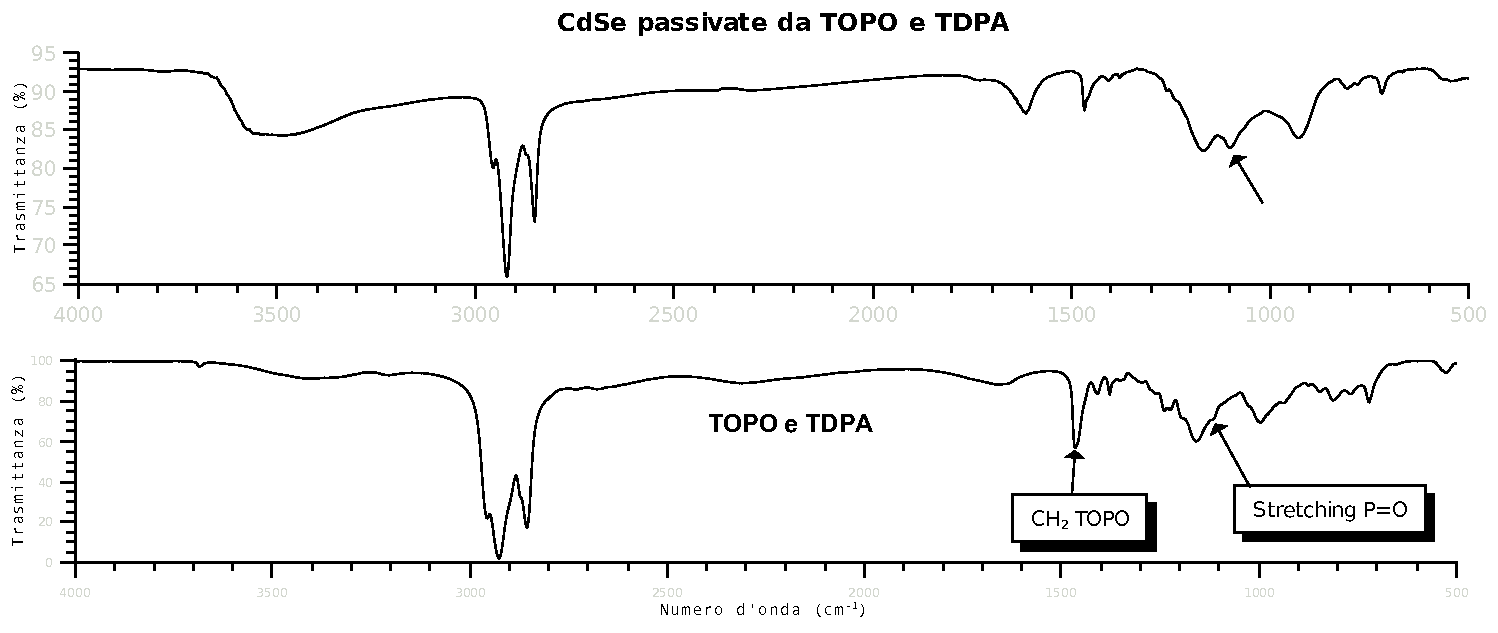
\includegraphics[width=.93\textwidth]{Immagini_Tesi/caratterizzazione/CdSe-TOPO_TDPA-IR-TOPO_TDPA.pdf}}
\caption{\footnotesize{In alto spettro FT-IR di NPs passivate con TOPO e TDPA\@. In basso spettro FT-IR di TOPO e TDPA puri.}
\label{fig:CdSe-TOPO_TDPA-IR-TOPO_TDPA}}
\end{figure}

\begin{figure}[!htb]
\centering{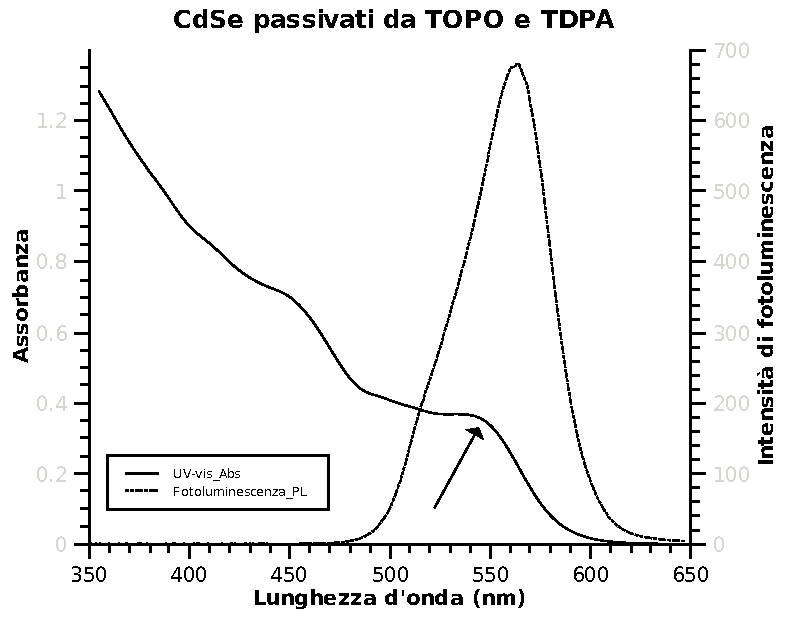
\includegraphics[width=.495\textwidth]{Immagini_Tesi/caratterizzazione/CdSe-TOPO_TDPA-in_toluene-UV_PL.pdf}
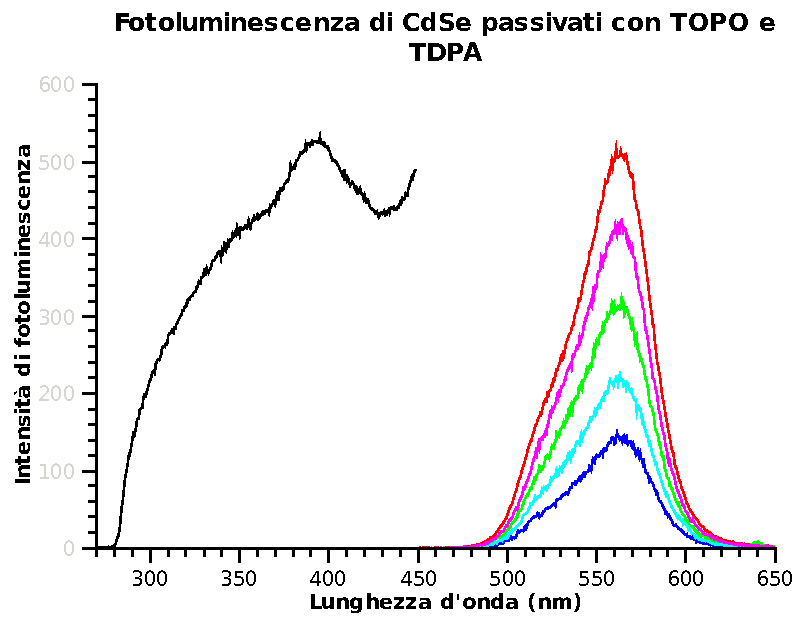
\includegraphics[width=.495\textwidth]{Immagini_Tesi/caratterizzazione/CdSe-TOPO_TDPA-movimentobanda-PL.pdf}\\
\makebox{\parbox[b]{.495\textwidth}{\centering{(a)}}}
\makebox{\parbox[b]{.495\textwidth}{\centering{(b)}}}}
\caption{\footnotesize{(a) Spettro UV-vis (---) e fotoluminescenza (- - -) di NPs di CdSe in toluene. (b) Fotoluminescenza con eccitazione a varie $\lambda$. La curva a $\lambda$ più basse è una scansione in eccitazione con $\lambda$ di osservazione a 563~nm. }}
\label{fig:CdSe-TOPO_TDPA-in_toluene-UV_PL-movimento}
\end{figure}

Dal picco dell'assorbimento eccitonico a maggiore lunghezza d'onda nello spettro UV-visibile (indicato da una freccia in~\ref{fig:CdSe-TOPO_TDPA-in_toluene-UV_PL-movimento}-(a)) possiamo ricavare la dimensione dei nanocristalli secondo la formula empirica~\cite{qd-CdSe-caratt}:
{\footnotesize{
\begin{equation}
D_{CdSe}=1.6122\cdot10^{-9}\lambda^4-2.6575\cdot10^{-6}\lambda^3+1.6242\cdot10^{-3}\lambda^2-0.4277\lambda+41.57
\label{eq:diametro}
\end{equation}
}}
Il picco in~\ref{fig:CdSe-TOPO_TDPA-in_toluene-UV_PL-movimento}-(a) si trova a circa 547~nm. Da questo e dall'Equazione~\ref{eq:diametro} si ricava un diametro di 3.0~nm. 

La fotoluminescenza è riportata in~\ref{fig:CdSe-TOPO_TDPA-in_toluene-UV_PL-movimento}-(b). Si osserva che il picco di emissione rimane centrato a 563~nm al cambiare di frequenze di eccitazione da 270~nm a 400~nm. 

Questo fatto significa che avviene solo una transizione e questo è indice di purezza del campione e dell'assenza di cadmio e selenio non reagito \cite{qd-CdSe-CdCl2}. 

Facendo una scansione in eccitazione tenendo fissa la lunghezza d'onda di osservazione si trova un massimo di a 393~nm.

L'analisi al DLS mostrata in~\ref{fig:AKT146-TOPO.CdSefilter-20100512}-(a) dà una dimensione media pesata sul volume di 2.2~nm.

Come si può vedere in~\ref{fig:AKT146-TOPO.CdSefilter-20100512}-(b) la media fatta sull'intensità del segnale strumentale è più alta a causa di impurezze o aggregati di nanoparticelle non filtrabili di diametro circa 15~nm.
\begin{figure}[!htb]
\centering{
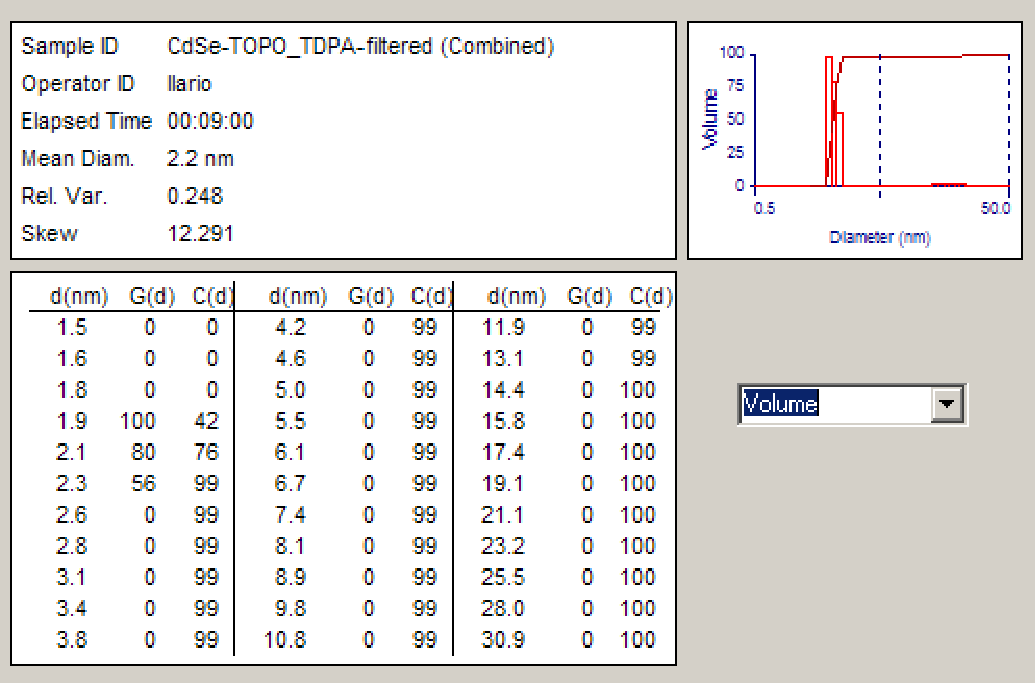
\includegraphics[width=.49\textwidth]{Immagini_Tesi/caratterizzazione/AKT146-TOPOCdSefilter-20100512-msd_summary.pdf}
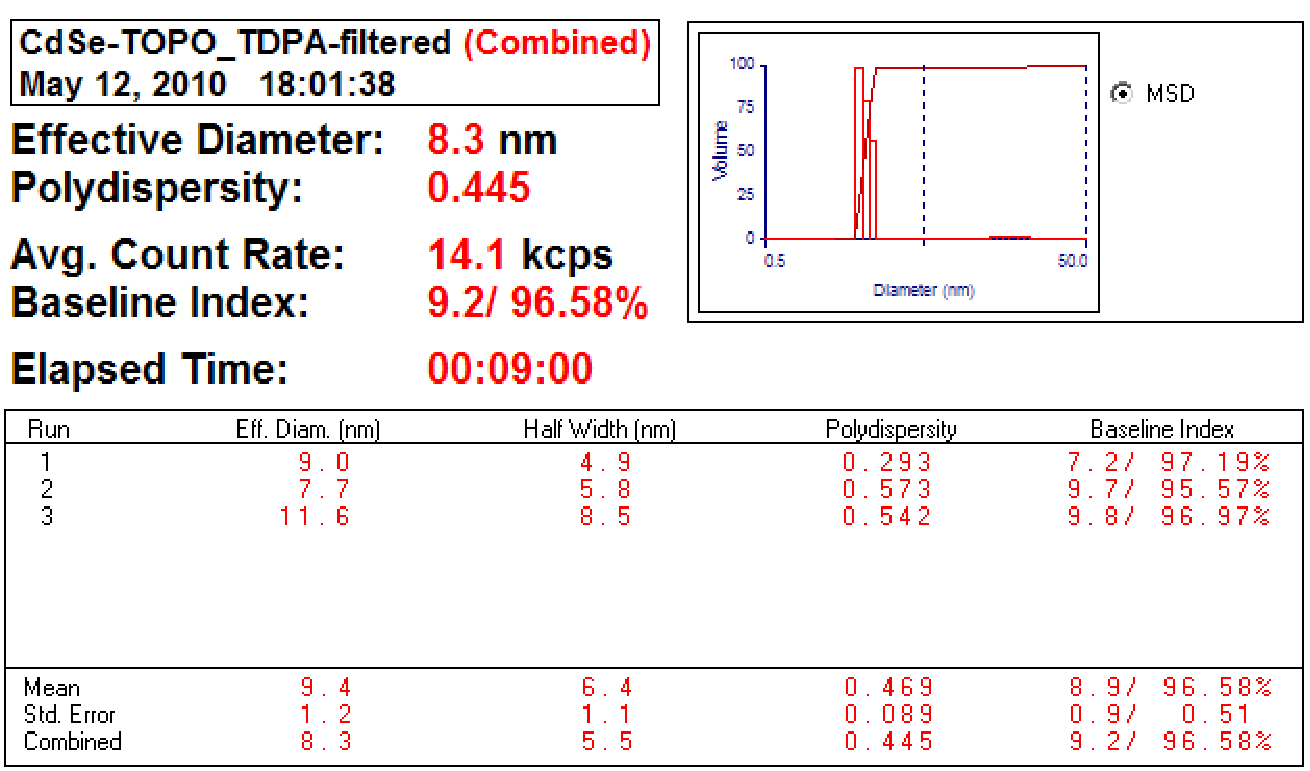
\includegraphics[width=.49\textwidth]{Immagini_Tesi/caratterizzazione/AKT146-TOPOCdSefilter-20100512-totale.pdf}\\
\makebox{\parbox[b]{.495\textwidth}{\centering{(a)}}}
\makebox{\parbox[b]{.495\textwidth}{\centering{(b)}}}
}
\caption{\footnotesize{(a) Media pesata sul volume di NPs di CdSe passivate con TOPO e TDPA in toluene (2.2~nm). \\(b) Media pesata sull'intensità del segnale e qualità del risultato (9.2/10).}}
\label{fig:AKT146-TOPO.CdSefilter-20100512}
\end{figure}

Nello spettro $^{31}$P \{$^1$H\} NMR in~\ref{fig:CdSe-TOPO_TDPA-P_NMR} si può riconoscere il segnale del fosforo legato alla nanoparticella a causa della sua caratteristica larghezza provocata {
dallo scambio tra la soluzione e l'ambiente non omogeneo vicino alla superficie della particella \cite{lig-CdSe-P}. Questo picco allargato può essere assegnato al TOPO \cite{lig-CdSe-P}. Non si osserva un secondo picco allargato per il TDPA perché quest'ultimo, avendo una interazione più forte con la superficie \cite{lig-CdSe-P}, non scambia con la soluzione e non è quindi possibile osservarlo (si trova costantemente in un ambiente quasi solido non analizzabile con tecniche convenzionali di NMR in soluzione).}

I picchi più stretti a $\delta$ 56.23, 44.54, 33.34~ppm sono da assegnare a nuclei di fosforo non legati alla superficie. Il picco a 56.23~ppm si può assegnare a TOPO libero ed il picco a 44.54~ppm può essere assegnato a acido P,P-diottil-fosfinico presente come impurezza nel TOPO commerciale e legante più debole di TOPO~\cite{lig-CdSe-P}.
\begin{figure}
\centering{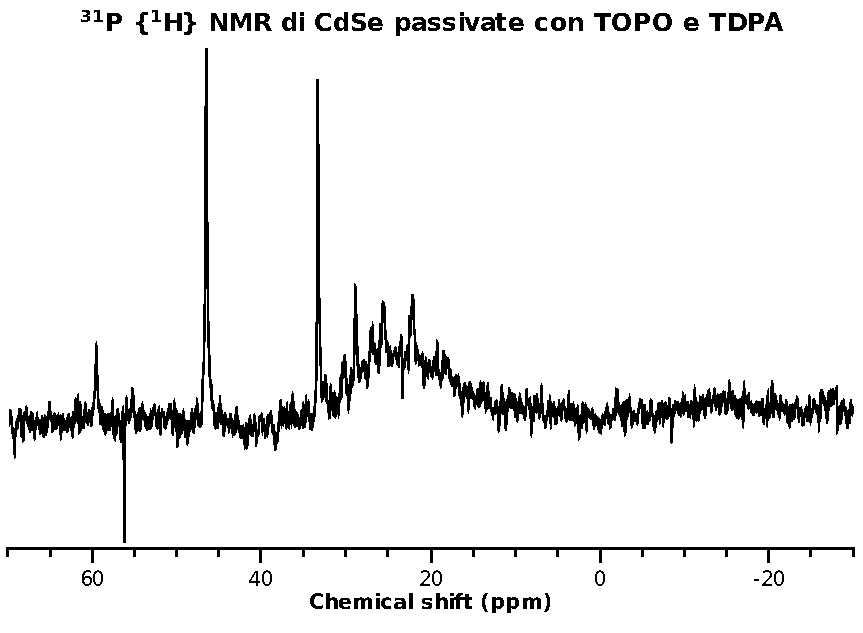
\includegraphics[width=.6\textwidth]{Immagini_Tesi/caratterizzazione/CdSe-TOPO_TDPA-P_NMR.pdf}}
\caption{\footnotesize{Lo spettro $^{31}$P \{$^1$H\} NMR di CdSe con TOPO e TDPA in CDCl$_3$ con una accumulazione di 16 ore (7345 transienti).}
\label{fig:CdSe-TOPO_TDPA-P_NMR}}
\end{figure}

{
In~\ref{fig:CdSe-TEM}-(a) è riportato un dettaglio dell'immagine registrata al microscopio ottico a trasmissione TEM\@. Da una analisi effettuata tramite apposito software si può vedere che le nanoparticelle sono monodisperse ed hanno una dimensione compresa tra 4.0~nm e 4.7~nm.

}
\begin{figure}[!htb]
\centering{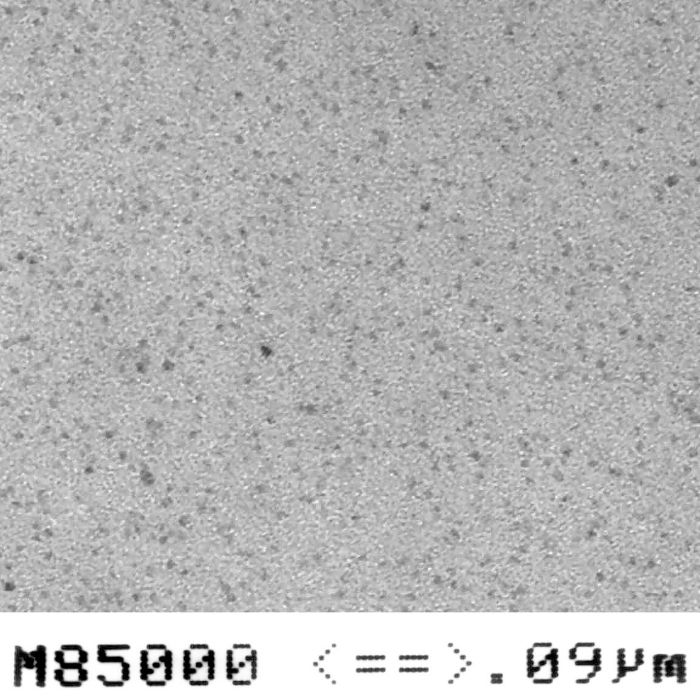
\includegraphics[width=.31\textwidth]{Immagini_Tesi/caratterizzazione/CdSe-TOPO_TDPA-TEM.jpg}
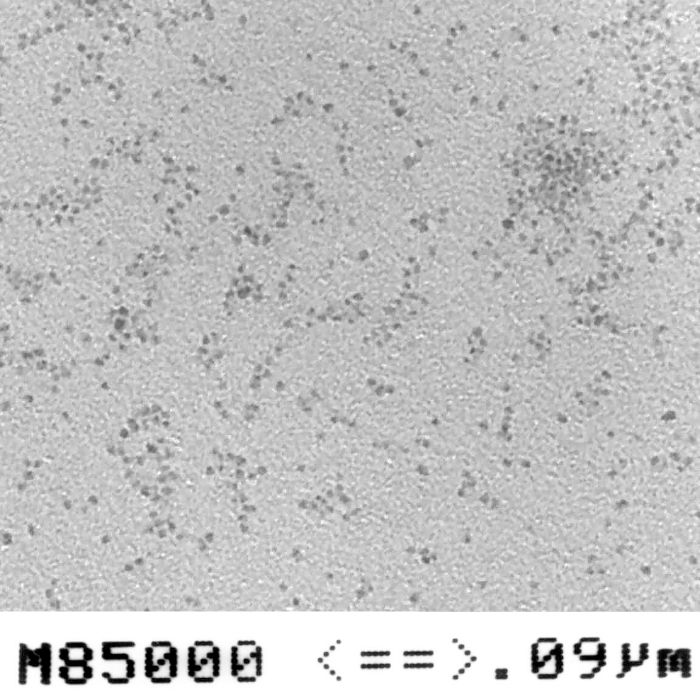
\includegraphics[width=.31\textwidth]{Immagini_Tesi/caratterizzazione/CdSe-pyr-TEM.jpg}
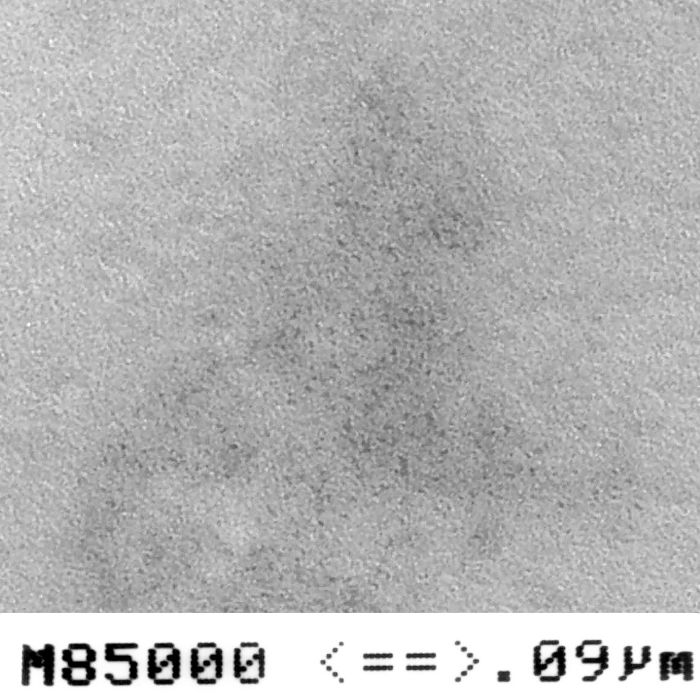
\includegraphics[width=.31\textwidth]{Immagini_Tesi/caratterizzazione/CdSe-P3HT-TEM.jpg}\\
\makebox{\parbox[b]{.31\textwidth}{\centering{(a)}}}
\makebox{\parbox[b]{.31\textwidth}{\centering{(b)}}}
\makebox{\parbox[b]{.31\textwidth}{\centering{(c)}}}}
\caption{\footnotesize{Immagine registrata al microscopio elettronico a trasmissione TEM di NPs di CdSe con: (a) TOPO e TDPA, (b) piridina, (c) polimero {\bf 7}. }}
\label{fig:CdSe-TEM}
\end{figure}
\section{Polimero coniugato}

Qui sono riportati i risultati della caratterizzazione $^1$H-NMR 
effettuata sul poli(3-esiltiofene) regioregolare terminato allile/Br \n{3}. 
\begin{figure}
\centering{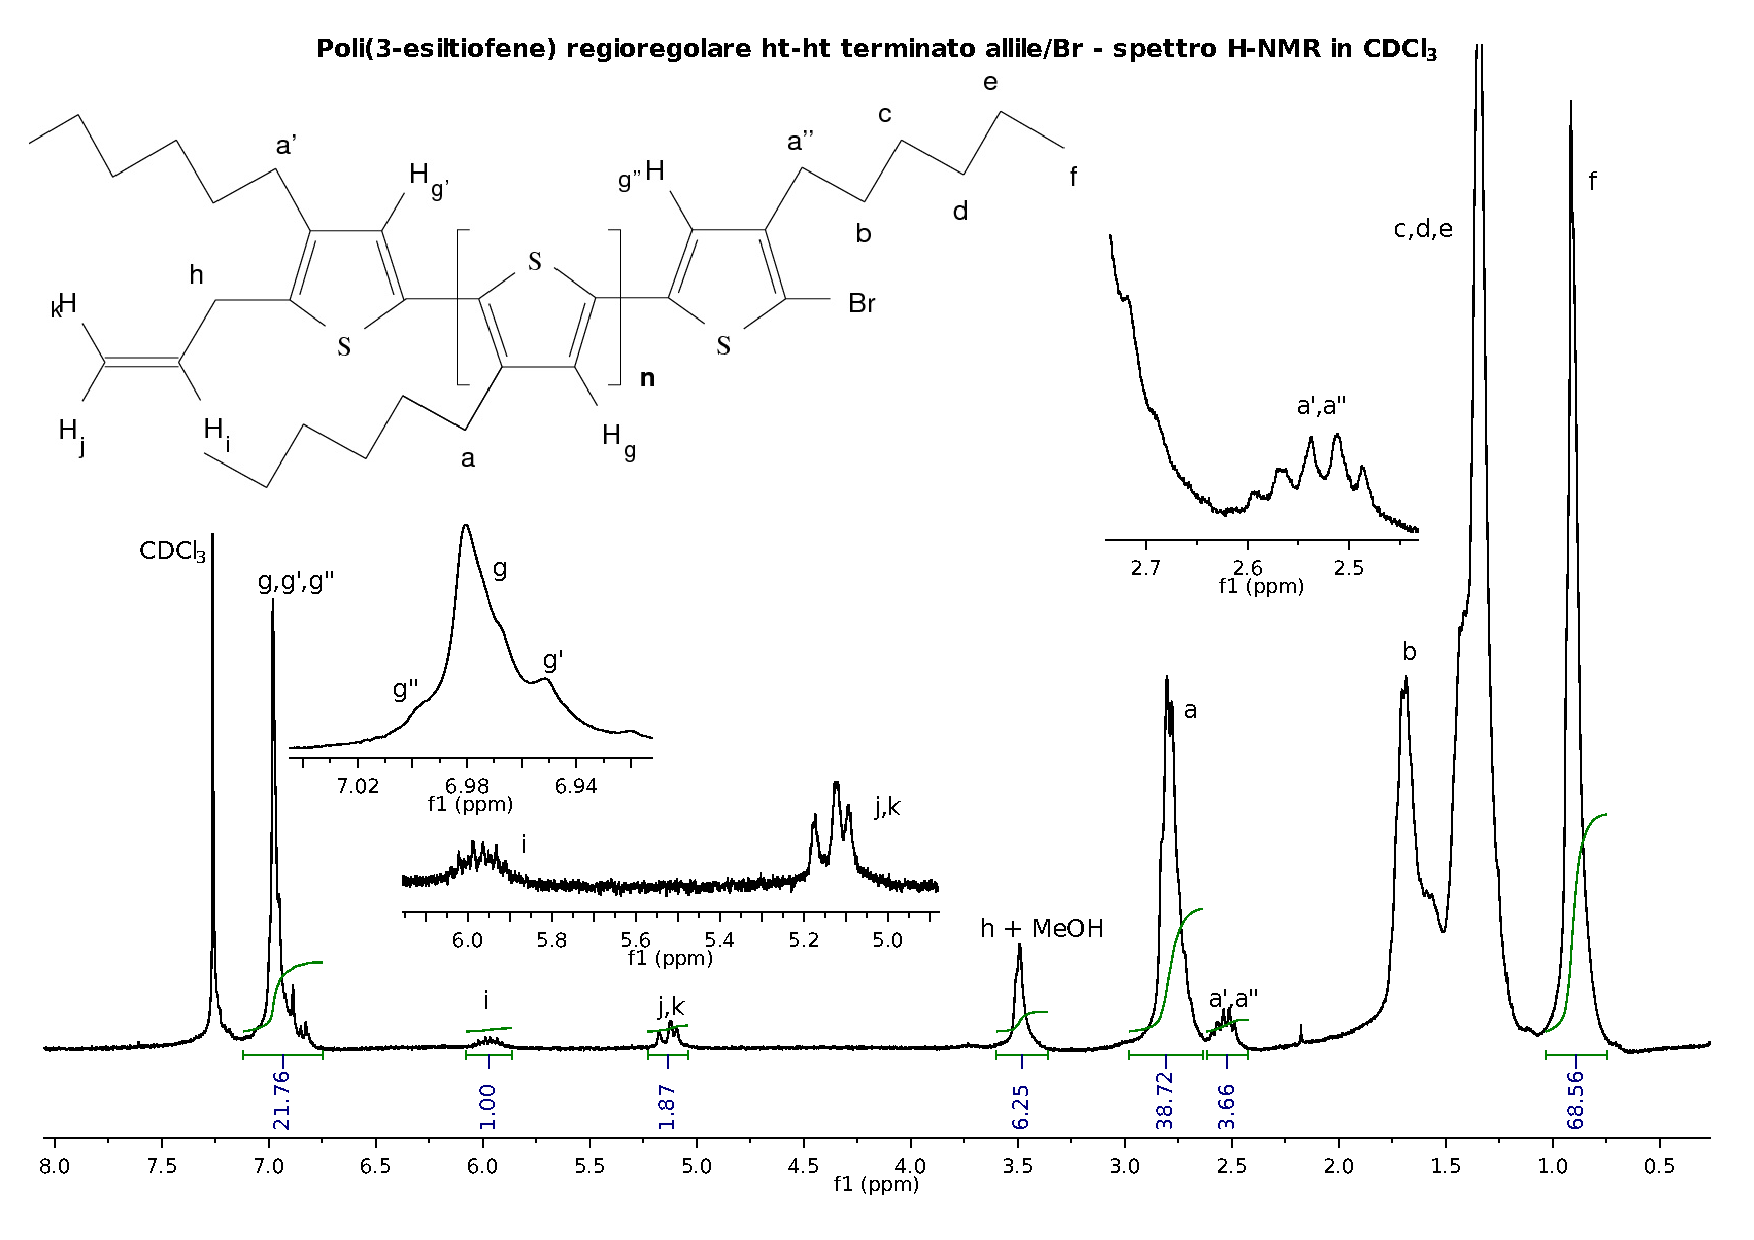
\includegraphics[width=.93\textwidth]{Immagini_Tesi/caratterizzazione/P3HT-HNMR.pdf}}
\caption{\footnotesize{Lo spettro $^1$H-NMR di poli(3-esiltiofene) regioregolare \emph{ht-ht} terminato allile/Br \n{3} in CDCl$_3$, 300MHz.}
\label{fig:P3HT-HNMR}}
\end{figure}

Dallo spettro $^1$H-NMR possiamo ottenere due importanti conferme: la conferma che il nostro polimero è regioregolare \emph{ht-ht} (vedi pagina \pageref{regio-htht}) e che sia monoterminato.

Il picco a 6.98~ppm viene attribuito al protone in posizione 4 sull'anello tiofenico. Questo può trovarsi in 4 distinti ambienti: \emph{ht-ht}, \emph{tt-ht}, \emph{ht-hh} e \emph{tt-hh} dando segnali a diversi \emph{chemical shifts}. Il picco a 6.98~ppm è riportato essere proprio del poli(3-esiltiofene) regioregolare \emph{head-tail-head-tail}~\cite{pol-p3ht-regio}. I \emph{chemical shifts} riportati per le altre regioregolarità sono: \emph{tail-tail-head-tail} 7.00, \emph{head-tail-head-head} 7.02 e \emph{tail-tail-head-head} 7.05~ppm.

Il picco a 2.80~ppm è proprio degli idrogeni {\bf a}, {\bf a'} e {\bf a''} sulla catena alifatica in posizione 3 sul tiofene. I protoni sulle 2 terminazioni danno tripletti, ma a \emph{chemical shift} leggermente diverso dal resto della catena.  Infatti si osservano i 2 tripletti isolati a 2.55~ppm. I tripletti non sono esattamente sovrapposti e danno forma ad un multipletto, questo conferma che {\bf a'} e {\bf a''} si trovano in ambienti diversi, perciò la terminazione è asimmetrica (la terminazione è l'unica differenza nel loro intorno, si ricordi da pagina \pageref{tail-tail} che entrambi i monomeri terminali sono legati al polimero col lato \emph{tail}).

Inoltre osservando le aree integrate e conoscendo l'assegnazione è possibile stimare la lunghezza del polimero. Il risultato di una tale stima è un polimero composto mediamente di 23 unità tiofeniche. 

\section{Modificazione della terminazione}
In questa sezione si riporta la caratterizzazione 
 del poli(3-esiltiofene) terminato allile/legante fosfonico protetto \n{6} ($^1$H-NMR, $^{13}$C-NMR, $^{31}$P NMR con disaccoppiamento protonico e NMR 2 bimensionale HMQC) e del poli(3-esiltiofene) terminato allile/legante fosfonico \n{7} (FT-IR, UV-vis, fotoluminescenza, $^1$H-NMR, $^{13}$C-NMR e $^{31}$P \{$^1$H\} NMR).

\begin{figure}
\centering{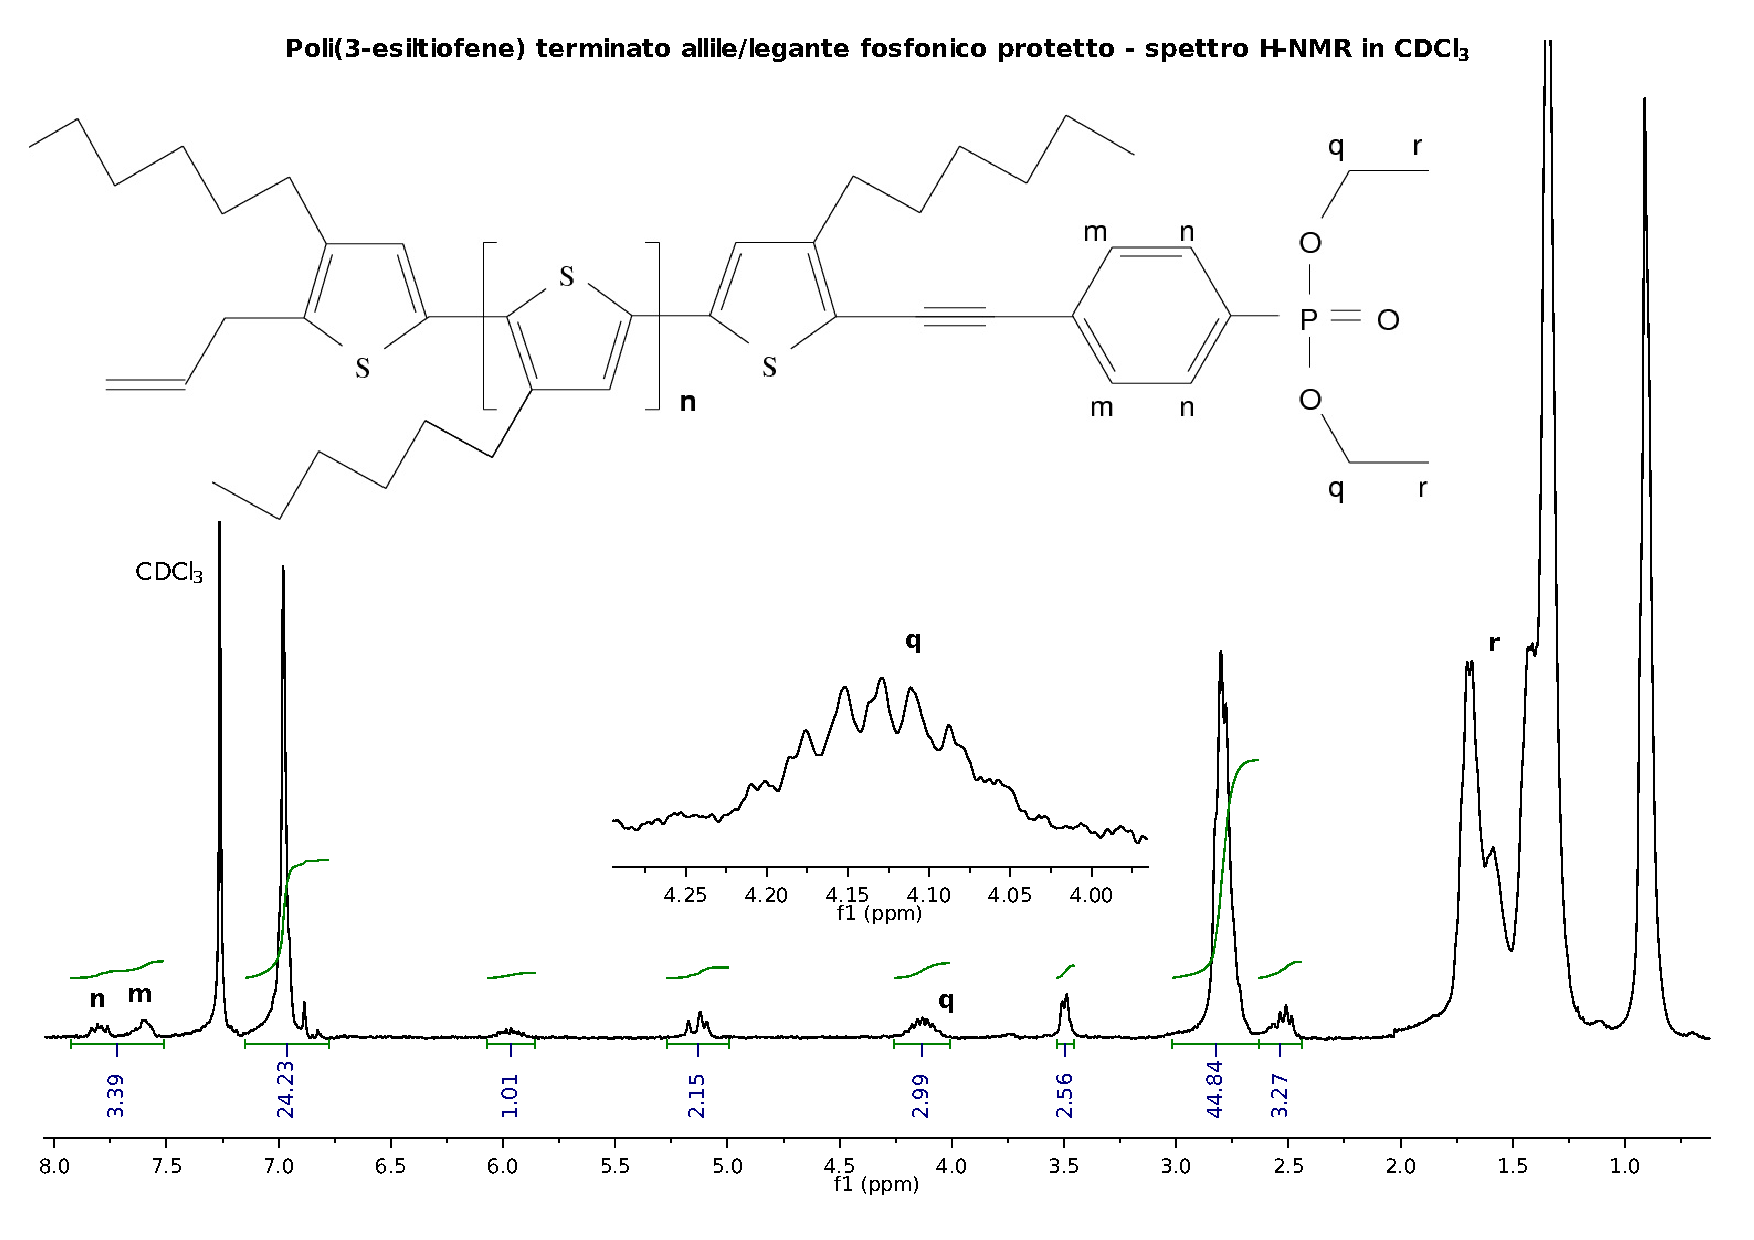
\includegraphics[width=.92\textwidth]{Immagini_Tesi/caratterizzazione/P3HT-leg-HNMR.pdf}}
\vspace{-15pt}
\caption{\footnotesize{Lo spettro $^1$H-NMR di poli(3-esiltiofene) terminato allile/legate fosfonico protetto in CDCl$_3$, 300MHz.}
\label{fig:P3HT-leg-HNMR}}
\end{figure}
Dallo spettro $^1$H-NMR di {\bf 6} riportato in~\ref{fig:P3HT-leg-HNMR} si possono osservare i picchi dell'anello benzenico e delle protezioni etile sul gruppo fosfato. L'area di questi picchi è circa 3 volte l'area corrispondente ad un singolo nucleo di H per una catena di circa 23 unità tiofeniche (sulla base dell'integrale della risonanza a 6.98~ppm) perciò la reazione ha avuto una buona resa ma non una resa quantitativa ed è presente del polimero {\bf 3} (che non viene rimosso dalle purificazioni effettuate). 

È stato registrato anche lo spettro $^{13}$C-NMR di {\bf 6} (75 MHz, \ce{CDCl3})  {
  riportato in~\ref{fig:P3HT-leg-CNMR}. I picchi sullo spettro $^{13}$C-NMR sono stati assegnati grazie all'ausilio di uno spettro bidimensionale HMQC di correlazione tra $^1$H e $^{13}$C direttamente legati. Questo spettro mostra i seguenti picchi: ($\delta_H$ - -  $\delta_C$, \ce{CDCl3}) 0.91 - - 14.0; 1.34 - - 31.9;  1.42 - - 22.9; 1.65 - - 30.8; 2.80 - - 29.6; 6.98 - - 128.8; 7.7~ppm - - 133.0~ppm. }
\begin{figure}
\centering{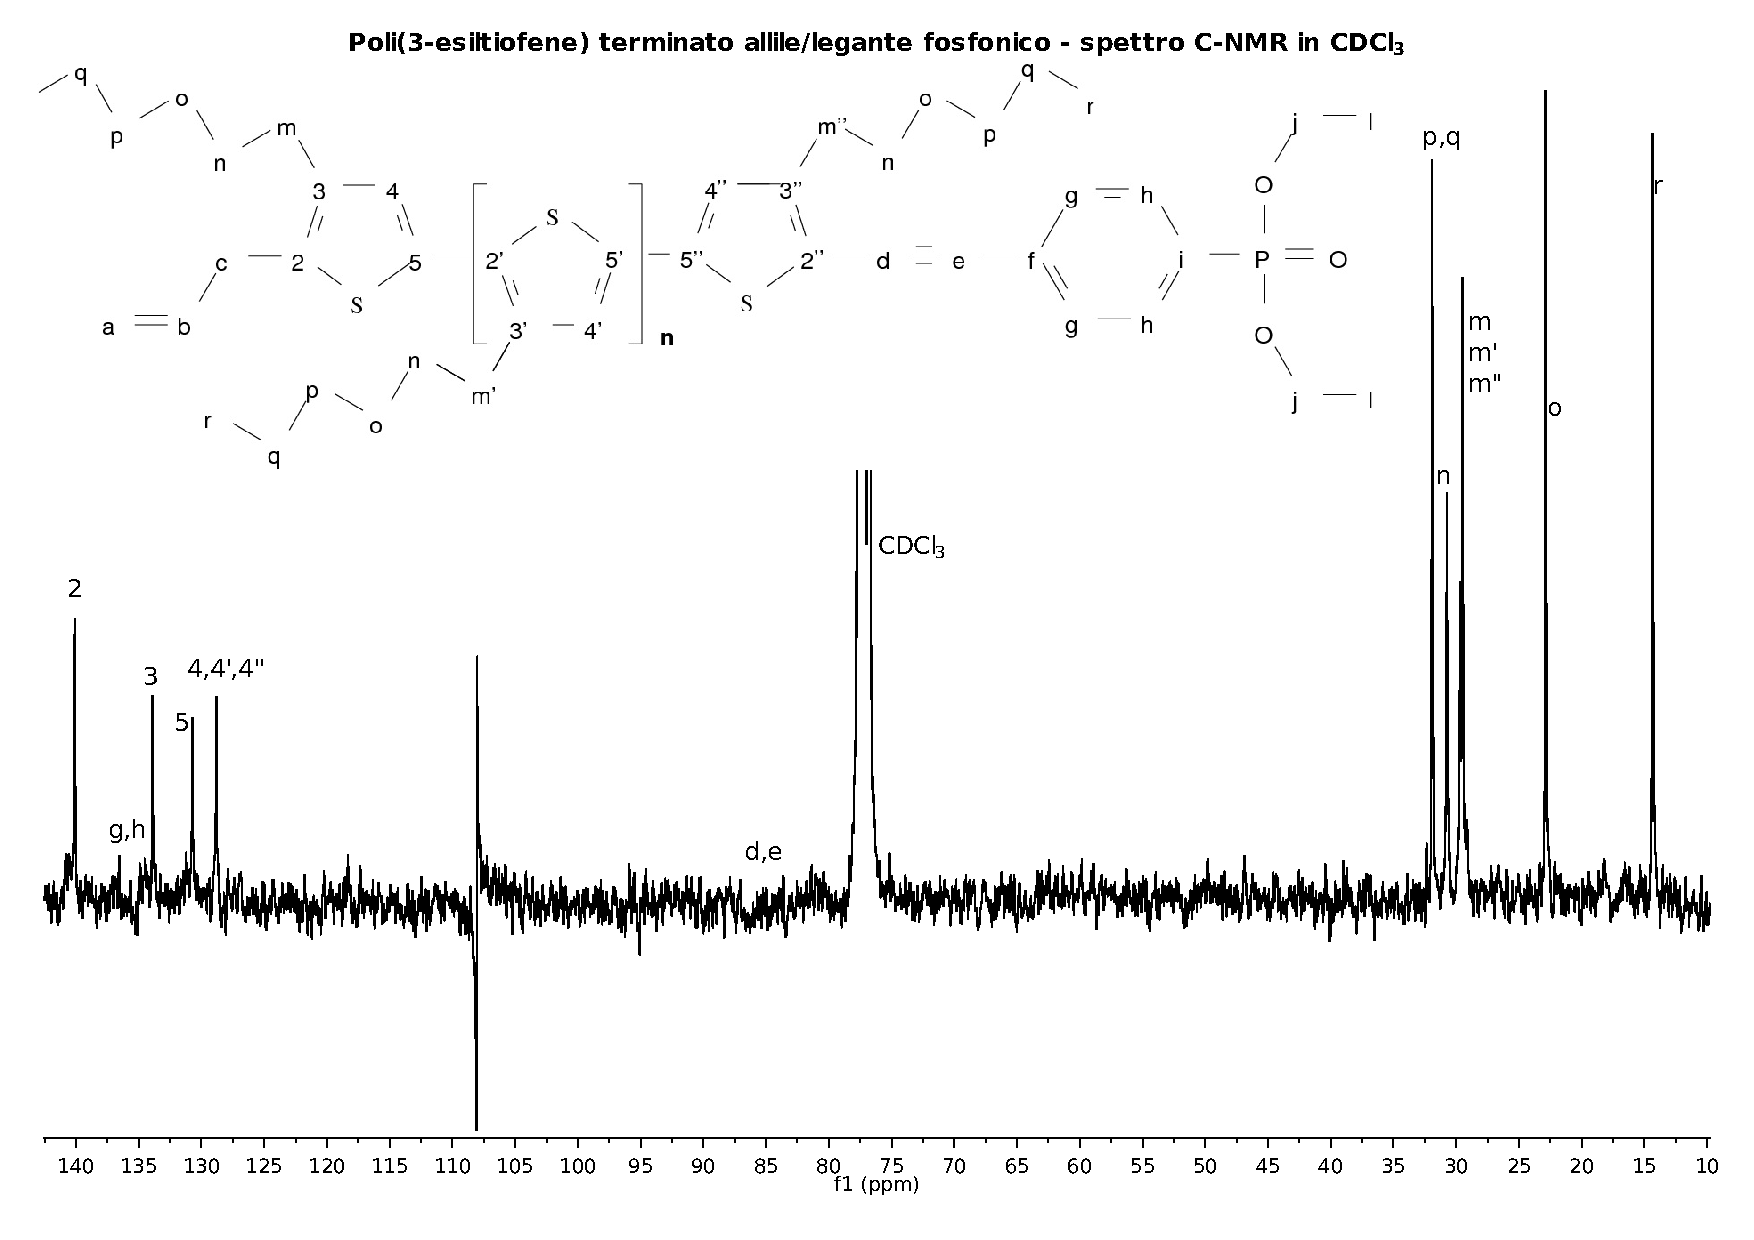
\includegraphics[width=.99\textwidth]{Immagini_Tesi/caratterizzazione/P3HT-leg-CNMR.pdf}}
\caption{\footnotesize{Lo spettro $^{13}$C-NMR di poli(3-esiltiofene) terminato allile/legate fosfonico protetto in CDCl$_3$, 75MHz.}
\label{fig:P3HT-leg-CNMR}}
\end{figure}

All'analisi $^{31}$P \{$^1$H\} NMR in \ce{CDCl3} è visibile solo il picco stretto a 15.79~ppm {
del fosforo sul gruppo legante. In questo caso non si ha allargamento del picco per formazione di micelle perché questa terminazione non è ancora abbastanza polare da formarne.}



\begin{figure}
\centering{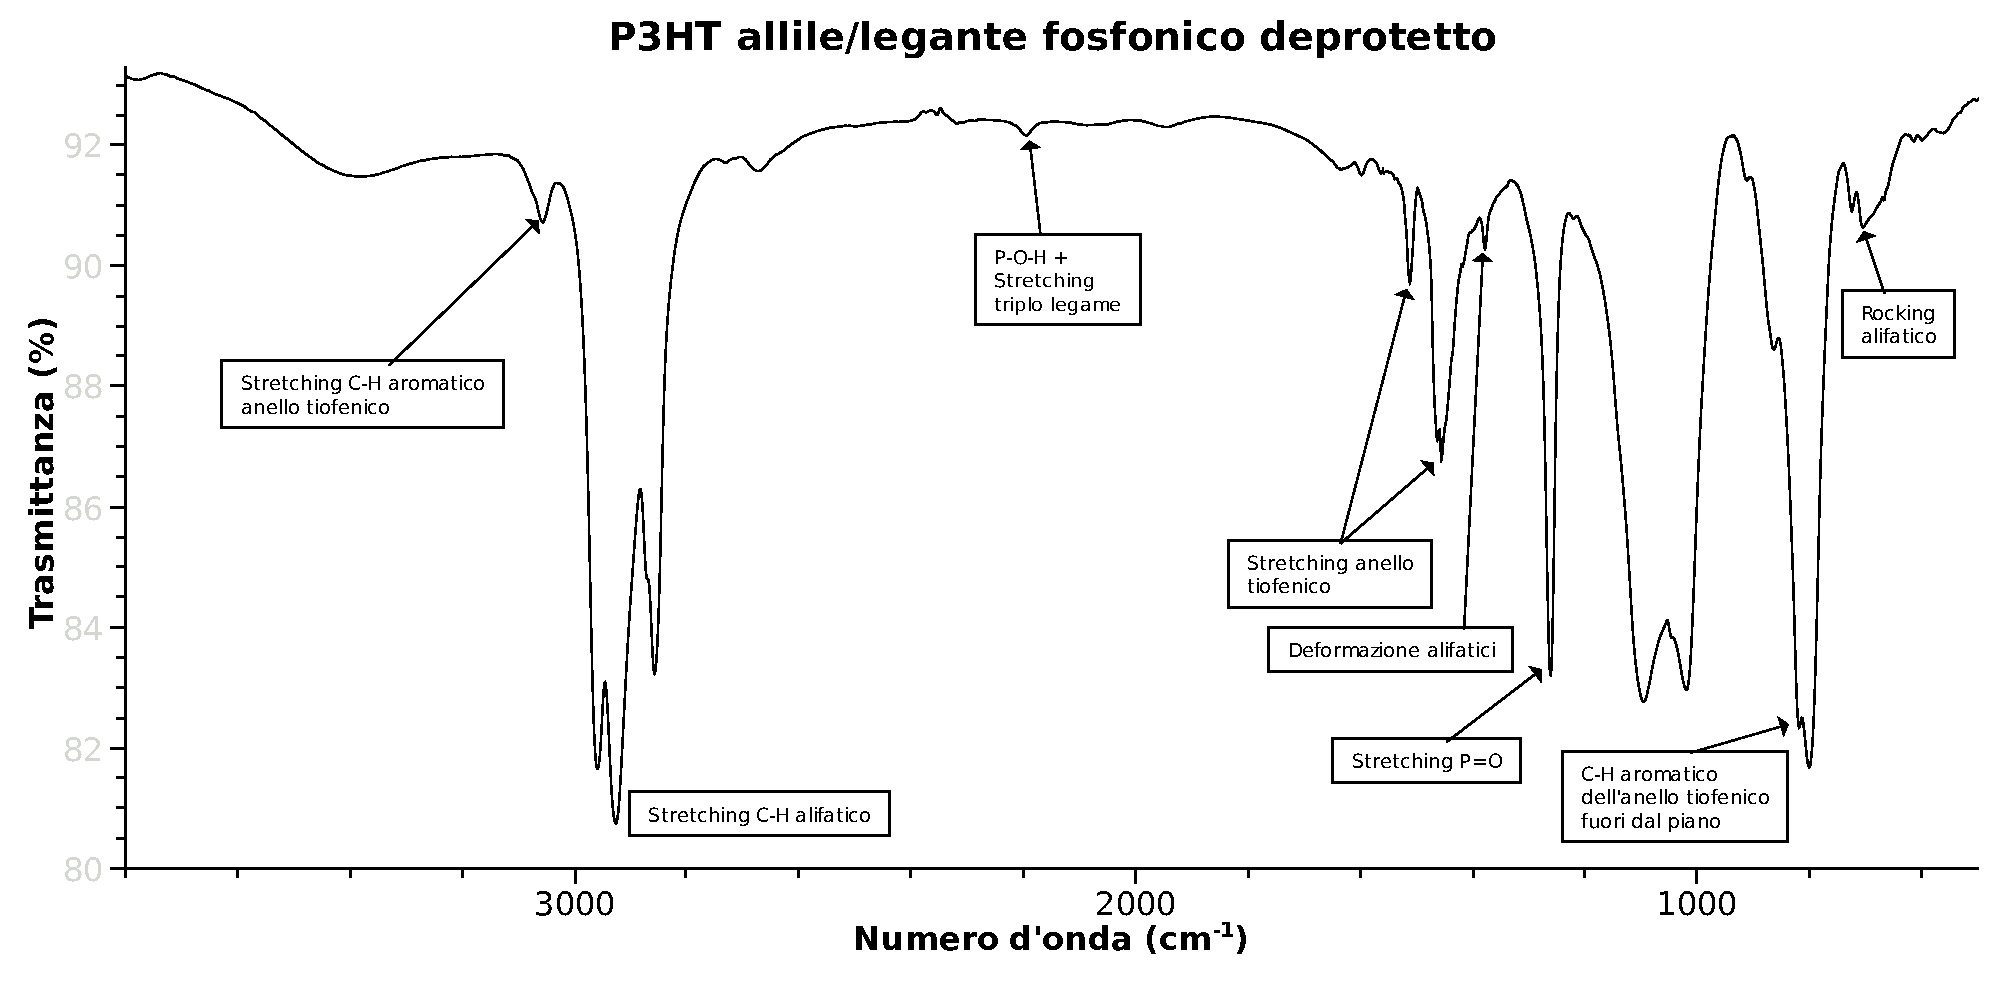
\includegraphics[width=.99\textwidth]{Immagini_Tesi/caratterizzazione/P3HT-leg-deprotetto-IR-assegnato.pdf}}
\caption{\footnotesize{Lo spettro FT-IR di {\bf 7} su pastiglia di KBr.}
\label{fig:P3HT-leg-deprotetto-IR}}
\end{figure}
Nello spettro FT-IR del poli(3-esiltiofene) terminato allile/legante fosfonico \n{7} riportato in~\ref{fig:P3HT-leg-deprotetto-IR} si osserva un piccolo picco a 2195~cm$^{-1}$ attribuibile a {
due segnali sovrapposti: il legame P-O-H del gruppo fosfonico ed il triplo legame presente tra la catena di polimero ed il legante. Più intenso} è il picco attribuibile allo \emph{stretching} P=O a 1262~cm$^{-1}$. Purtroppo gli altri picchi caratteristici del legante vengono coperti dall'assorbimento del polimero, {
ben più intenso a causa della ripetizione dei monomeri risultante in una magnificazione dei loro assorbimenti.}
  


\begin{figure}
\centering{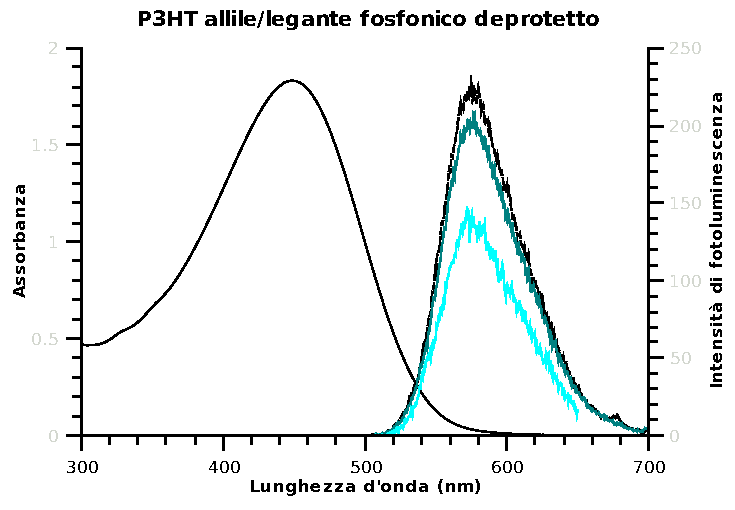
\includegraphics[width=.7\textwidth]{Immagini_Tesi/caratterizzazione/P3HT-leg-deprotetto-UV-PL.pdf}}
\caption{\footnotesize{Spettro di assorbimento ({\bf \large{---}}) e di fotoluminescenza di {\bf 7} in cloroformio a varie lunghezze d'onda: 270~nm ({\Large{{\bf{\color{cyan}---}}}}), 340~nm ({\bf \normalsize{- - -}}), 350~nm ({\Large{{\bf{\color{blue}---}}}}).}
\label{fig:P3HT-leg-deprotetto-UV-PL}}
\end{figure}
Lo spettro di assorbimento UV-vis e lo spettro di fotoluminescenza di {\bf 7} sono riportati in~\ref{fig:P3HT-leg-deprotetto-UV-PL}. Lo spettro UV-vis ha un massimo di assorbimento centrato a 449~nm. In letteratura \cite{pol-p3ht-regio} si trova che per il poli(3-esiltiofene) regiorandom si ha il picco di assorbimento a 428~nm. La posizione del picco a $\lambda$ maggiori indica una maggiore coniugazione che deriva dalla regioregolarità.

Il picco di emissione di fotoluminescenza si trova a 576~nm e non varia in lunghezza d'onda eccitando nell'intervallo tra 270~nm e 400~nm con un massimo in intensità a 341~nm.  

Lo spettro $^1$H-NMR di {\bf 7} differisce dallo spettro di {\bf 6} essenzialmente per la mancanza del multipletto a 4.12~ppm attribuito agli idrogeni metilenici del gruppo etile protezione del gruppo fosfato. Un'altra importante differenza dallo spettro precedente sta nella assenza dei picchi propri degli idrogeni aromatici sul legante. Una possibile giustificazione di questa mancanza sta nella formazione di strutture micellari inverse. Queste si possono formare per la presenza del gruppo legante fosfonico deprotetto polare. Il legante potrebbe quindi trovarsi in una zona con caratteristiche di mobilità ridotta tali da renderlo non osservabile con tecniche convenzionali di NMR in soluzione \cite{lig-micelle-nmr2}. Registrando lo stesso spettro $^1$H-NMR a temperatura maggiore (35°C) non sono state osservate differenze. 

È stato registrato lo spettro $^{13}$C-NMR di {\bf 7}: (75 MHz, \ce{CDCl3}): $\delta$ 1.27, 14.37, 22.90, 29.51, 29.71, 30.75, 31.94, 116.32, 128.81, 130.70, 133.91, 136.54, 140.10~ppm. 

Lo spettro $^{31}$P \{$^1$H\} NMR di {\bf 7} registrato a 40°C è risultato molto diverso dallo spettro di {\bf 6}. Il picco a 15.79~ppm non è più presente mentre si possono osservare dei segnali allargati, tipici {
di una breve permanenza in ambiente liquido con un veloce scambio in un ambiente non uniforme come quello di una struttura micellare \cite{lig-micelle-nmr2}.}
\begin{figure}
\centering{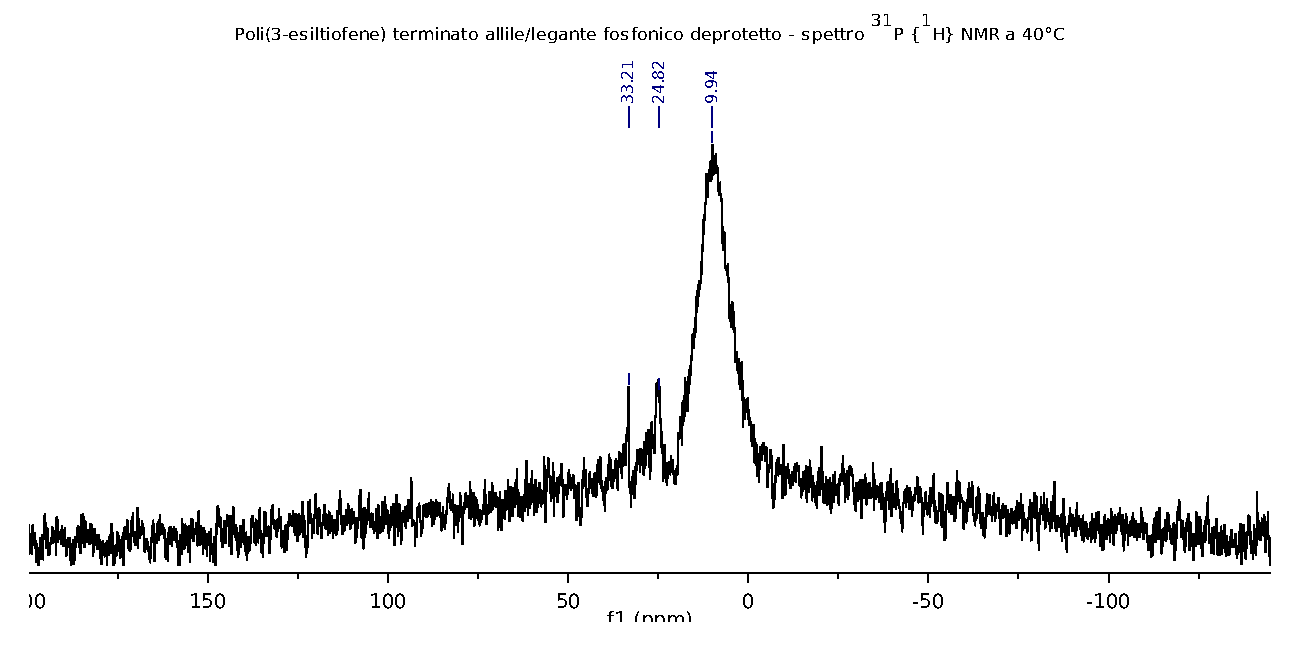
\includegraphics[width=.8\textwidth]{Immagini_Tesi/caratterizzazione/P3HT-leg-PNMR.pdf}}
\caption{\footnotesize{Spettro $^{31}$P \{$^1$H\} NMR di {\bf 7} in \ce{CDCl3} a 40°C con una accumulazione di 18 ore (8624 transienti).}
\label{fig:P3HT-leg-PNMR}}
\end{figure}


\section{Scambio di leganti}

In questa sezione si espongono i risultati della caratterizzazione dello scambio di leganti sulle nanoparticelle (NPs) di CdSe eseguito in successione prima con piridina e poi con il polimero {\bf 7}. 
Del primo prodotto di scambio di leganti sono stati registrati gli spettri FT-IR, UV-vis, fotoluminescenza, $^1$H-NMR, $^{31}$P \{$^1$H\} NMR e TEM\@.  Il prodotto del secondo scambio di leganti è stato caratterizzato registrando gli spettri 
UV-vis, fotoluminescenza, {
  $^{31}$P \{$^1$H\} NMR e TEM.}

Nello spettro FT-IR delle NPs passivate da piridina {
 sono ancora presenti i picchi dovuti alle catene alifatiche di TOPO e di TDPA}.

Lo spettro UV-vis mostra la posizione del primo picco eccitonico a 544~nm.
Questo dato inserito nell'Equazione~\ref{eq:diametro} dà un diametro di 2.9~nm, compatibile col dato ricavato a pagina \pageref{eq:diametro} per le NPs appena sintetizzate. Perciò le particelle non si sono unite a dare aggregati. 

L'analisi di fotoluminescenza sulle nanoparticelle passivate con piridina ha dato un solo picco allargato ed estremamente debole a 555~nm.

Nello spettro $^1$H-NMR 
sono presenti 3 picchi larghi attribuibili alla piridina ($\delta$ 8.62, 7.68, 2.29~ppm). Il fatto che questi picchi siano allargati testimonia lo scambio di piridina tra la soluzione e un ambiente anisotropico come la superficie di una nanoparticella. Inoltre nello spettro sono visibili i picchi di TOPO e di TDPA ancora presenti in soluzione (che si ritiene quindi possano essere efficacemente rimossi con la successiva purificazione).

Infatti nello spettro $^{31}$P \{$^1$H\} NMR di CdSe passivato con piridina non è visibile, nemmeno dopo 11 ore di accumulazione (5485 transienti),  {
il picco allargato che precedentemente era stato attribuito al TOPO, a indicazione di una efficace e pressoché quantitativa sostituzione di quest'ultimo dalla superficie da parte della piridina.} Lo spettro presenta picchi stretti a $\delta$ 56, 23 e 7~ppm. I primi due possono essere attribuiti \cite{lig-CdSe-P} rispettivamente a TOPO ed a TDPA liberi ossia non legati a nanoparticelle.

{
 Nell'immagine registrata al TEM (\ref{fig:CdSe-TEM}-(b)) si osservano nanoparticelle con dimensioni da 3.0~nm a 5.0~nm. Le particelle non sono monodisperse come nella precedente immagine al TEM ma non si ha nemmeno una evidente formazione di aggregati che risulterebbero come grandi macchie nere dovute alla sovrapposizione di NPs anche lungo l'asse $z$ perpendicolare al piano di osservazione. }

Nello spettro UV-vis del prodotto del secondo scambio di leganti il picco a maggiore lunghezza d'onda è dovuto ai nanocristalli e si trova a 550~nm. Utilizzando l'Equazione~\ref{eq:diametro} si ricava un diametro di 3.0~nm, sostanzialmente invariato dalle precedenti misurazioni, ad ulteriore conferma della sostanziale assenza di aggregazione. È presente inoltre una seconda banda di assorbimento con massimo a 447~nm attribuibile al polimero coniugato. Perciò sostanzialmente lo spettro UV-vis è risultato la somma dei due spettri dei precursori.

Il massimo di emissione di fotoluminescenza cambia {
 leggermente } lunghezza d'onda in funzione della $\lambda$ di eccitazione, risultando inoltre tutt'altro che la somma delle bande di emissione di fluorescenza dei due precursori. È riportata in letteratura \cite{lig-PL-quenching} la diminuzione dell'intensità del picco d'emissione delle nanoparticelle indicativa del minore confinamento quantico, diminuito dal contatto elettrico con il polimero coniugato. {
 Infatti la posizione del picco di emissione (573-581~nm) risulta più simile a quella del polimero (576~nm) che delle NPs passivate con TOPO e TDPA (563~nm)}.

{
Lo spettro $^{31}$P \{$^1$H\} NMR con accumulazione di 14 ore (1745 transienti) mostra due picchi molto stretti a 3.59 ed a -1.08~ppm forse non significativi e nessun picco allargato. Lo spettro $^{31}$P \{$^1$H\} NMR registrato a 35°C non presenta significative differenze. L'assenza del picco largo presente nello spettro di {\bf 7} (riportato in~\ref{fig:P3HT-leg-PNMR}) è significativa dell'assenza di polimero legante libero di formare micelle (o comunque presente in concentrazione molto minore del campione analizzato di {\bf 7} puro, tanto da risultare sotto la sua concentrazione micellare critica). Perciò tutto (o quasi) il polimero aggiunto si ritiene debba essere legato alle NPs. Inoltre il fatto che non si abbia nessun picco allargato indica l'assenza di uno scambio dinamico sulla superficie della NP ed una permanenza del gruppo legante sulla superficie delle NPs. Infatti quando il gruppo fosfonico si trova nell'ambiente anisotropo quasi solido della superficie non se ne può osservare il segnale \cite{lig-micelle-nmr2}. Se ne conclude che il legame dev'essere forte.}

{
L'immagine registrata con il microscopio elettronico a trasmissione in~\ref{fig:CdSe-TEM}-(c) non è chiara come le precedenti due immagini a causa della presenza del polimero. Ciononostante si può osservare che le nanoparticelle sono disperse nella matrice di polimero e non sono aggregate se non in blocchi di piccola estensione di cui si può solamente intuire la presenza nell'immagine.}

